\subsection{Glühemission einer Diode}
\label{sub:glühemission_einer_diode}
  Um freie Elektronen zu erzeugen muss man in Materialien an Atome gebundene Elektronen Energie zuführen. Dazu gibt es verschiedene Möglichkeiten:
  Durch schnelle Teilchen aus dem inneren eines Materials (thermisch) oder von außen (Sekundäremission), durch Photonen oder starke elektrische Felder.
  In diesem Versuch wird die thermische Emission untersucht (auch Glühemission, Richardson-Effekt).
  \par
  In diesem Versuch wird der Effekt innerhalb einer Diode untersucht. Diese besteht aus einem evakuierten Glaskolben, in den zwei Elektroden eingeschmolzen sind: Die Kathode kann geheizt werden und dient folglich als Elektronenquelle. Wird zwischen Kathode und Anode ein Feld angelegt, so kann der Strom in Abhängigkeit der angelegten Spannung gemessen werden.

  \begin{figure}[H]
    \centering
    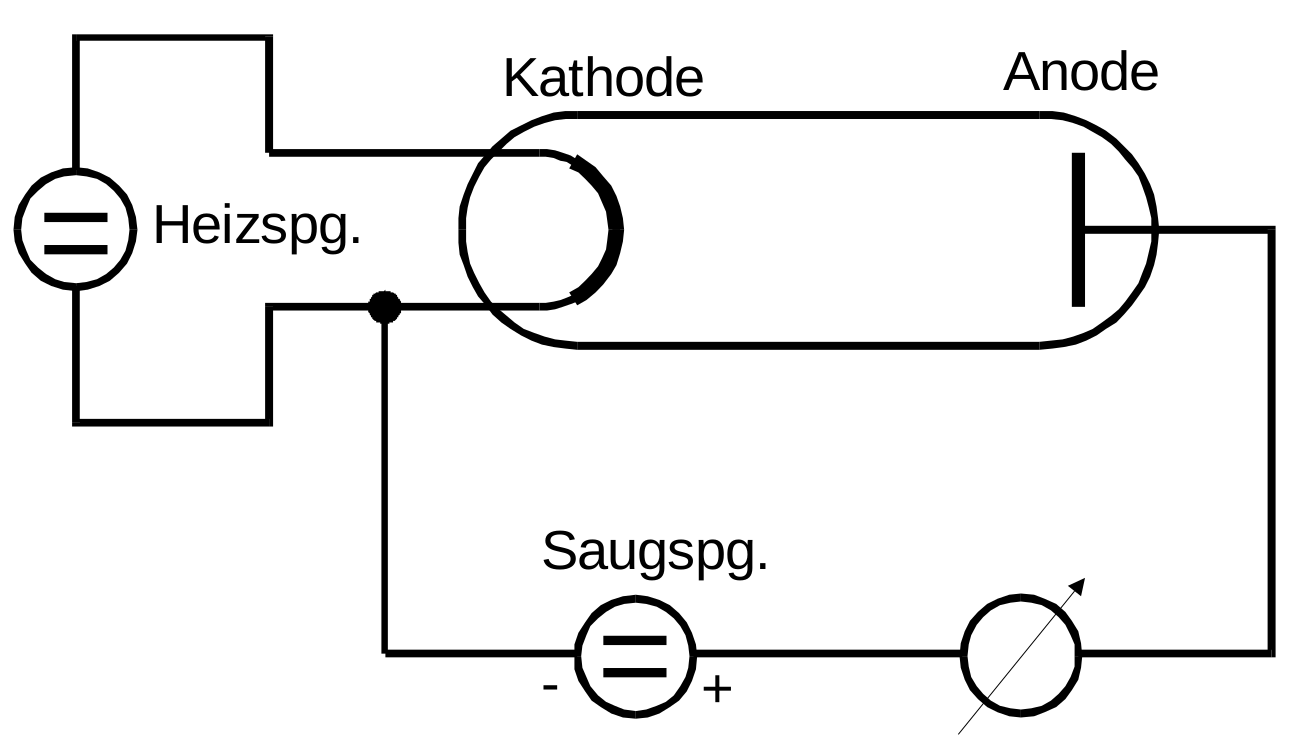
\includegraphics[width=\textwidth]{../figures/diode_aufbau.png}
    \caption{Schematischer Aufbaue und Beschaltung einer Diode.}
    \label{fig:_figures_diode_aufbau_png}
  \end{figure}

  Ziel ist es, die Strom-Spannungs-Kennlinie einer solchen Diode zu bestimmen.


\subsection{Richardson-Effekt}
\label{sub:richardson_effekt}
  Die in einem Metall am schwächsten gebundenen Elektronen (Leitungselektronen) können sich frei innerhalb des Metalls bewegen\footnote{Daher rührt die gute elektrische Leitfähigkeit.}. Beim Verlassen des Ionengitters wird dieses jedoch positiv geladen. Ein Elektron muss also die durchschnittliche Gitterenergie $-W_a$ aufbringen, um in den Außenraum treten zu können.
  \par
  Um dort zu einer freien Ladung zu werden muss sie ferne genug Energie besitzen, um aus dem Feld der Spiegelladung zu entkommen ($E_s = -e^2/(16 \pi \varepsilon_0 x)$). Beide Arbeiten werden nach \emph{Sommerfeld} zu einem Kastenpotential der Höhe $e \Phi$ vereinfacht\footnote{Dabei ist $e$ die (negative) Elementarladung.}. Dieses hat den Transmissionskoeffizienten $t$\footnote{Im weiteren wird $t\approx 1$ angenommen. I.A. ist dieser aber abhängig von der Form und Größe der Potentiale.}. Im klassischen Sinne ist $e \Phi$ die Verdampfungswärme eines Elektrons.

  Zunächst besitzen die Elektronen nur thermische Energie. Ist diese größer als $e\Phi$ so können sie beim Erreichen der Oberfläche zu freien Elektronen werden. Die Energieverteilung der Elektronen im Metall wird durch die \emph{Fermi-Verteilung} beschrieben, die anders als die sonst für thermische Prozessen angenommene Boltzmann-Verteilung\footnote{Für große Energien gehen beide Verteilungen ineinander über.} berücksichtigt, dass jeder mögliche Energiezustand nur von zwei Elektron besetzt werden kann (Pauli-Verbot):
  \begin{align}\label{equ:fermi}
    N(W) = 4\pi (\frac{2 m}{h^2})^{1.5} \frac{W^{0.5}}{e^{(W-W_F)/{kT}}+1}
  \end{align}
  Dabei beschreibt
  \begin{align}\label{equ:fermi_energy}
      W_F = \frac{\hbar^2}{2m} (3\pi^2 n)^{2/3}
   \end{align}
  die Fermi-Energie. Dies ist die höchste Energie, die ein gebundenes Fermion annehmen kann, wenn sich das System im Zustand niedrigster Energie befindet (d.h. bei $T=\SI{0}{\K}$). $k$ ist die Boltzmannkonstante, $T$ die Temperatur, $m$ die Masse eines Elektrons.
  \par

  \begin{figure}[H]
    \centering
    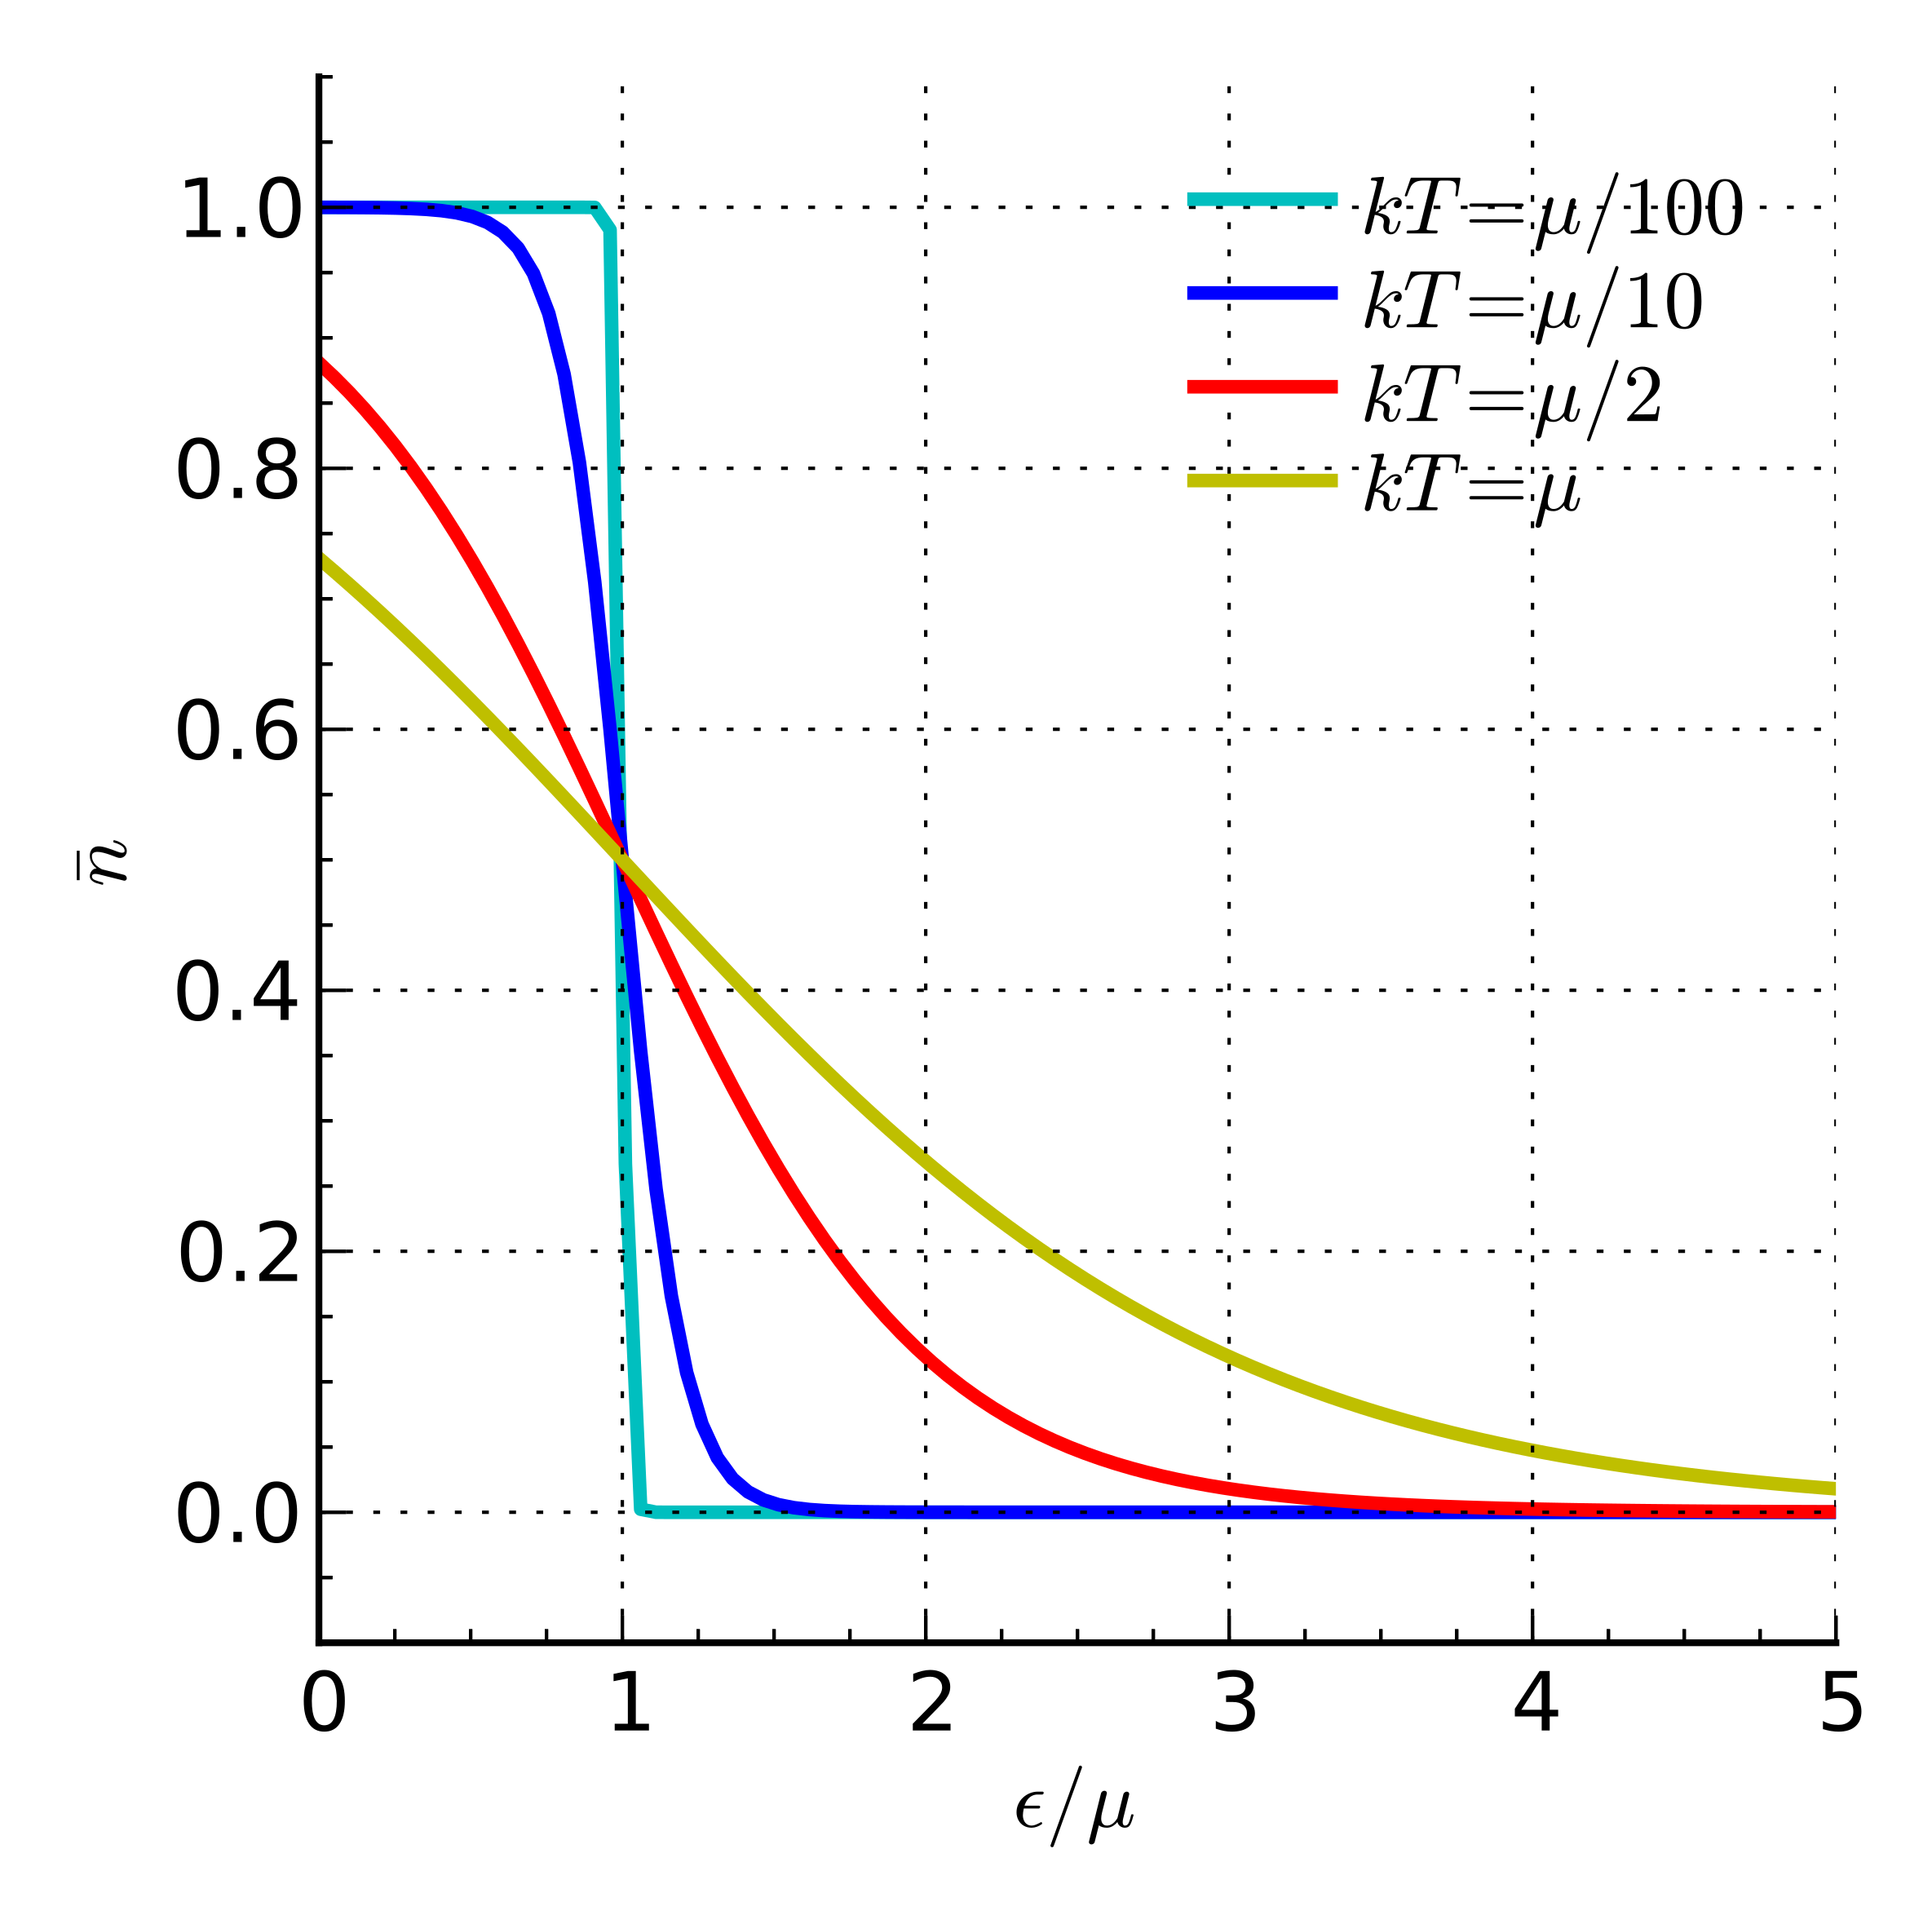
\includegraphics[width=0.4\textheight]{../figures/fermi.png}
    \caption{Fermiverteilung für verschiedene Temperaturen. Deutlich sichtbar ist die Lage Fermienergie im Punkt $(1,1.5)$. [Wiki]}
    \label{fig:aufbau}
  \end{figure}

  Exakt gilt diese Verteilung nur im thermischen Gleichgewicht, die Fermi-Statistik liefert aber auch im Fall, in dem Elektronen durch ein äußeres Feld entfernt werden, noch Ergebnisse mit ausreichender Genauigkeit.
  In diesem symmetrischen Problem ist der Elektronenfluss in Richtung der Oberflächennormale überall gleich; somit gibt
  \begin{align}\label{equ:electronflux}
    j = e \integral{N(W) v_z}{W}{0}{\infty}
  \end{align}
  den Elektronenstrom an. Dabei ist $v_z$ die Geschwindigkeit eines Elektrons senkrecht zur Oberfläche.

  Dieses Integral kann durch die Identität $W=\frac{1}{2} m \vec{v}^2$ in drei Integrale der Geschwindigkeitskomponenten aufgeteilt werden. Dabei umfasst das Integralgebiet für die $x$,$y$-Komponenten ganz $\mathds{R}$, für die $z$-Komponente jedoch nur $[(2(W_F+e \Phi)/m)^{0.5},\infty]$. Dies ergibt sich aus folgender Überlegung:
  \par
  Ein austretendes Elektron muss in $z$-Richtung die Austrittsarbeit $e\Phi$ aufbringen können, um einen ungebundenen Zustand zu erreichen. Es besitzt bereits $W_F$. Daraus folgt
  \begin{align}\label{equ:minwork}
    E   &= W_F + e\Phi = \frac{1}{2} m v_z^2\\
    v_z &= (2(W_F+e \Phi)/m)^{0.5} \;.
  \end{align}
  \par

  Damit ergibt sich für den austretenden Elektronenstrom
  \begin{align}\label{equ:richardson}
    j_R = (4\pi m e k^2/h^3) T^2 e^{-e\Phi/{kT}}\;.
  \end{align}



\subsection{Langmuir-Shottky-Raumladungsformel}
\label{sub:shottky_langmuir_strom}
  Der aus der im vorherigen Abschnitt bestimmten Stromdichte folgender Strom wird in einer Diode nur erreicht, wenn alle Ladungsträger, die aus der Kathode austreten, von der Anode direkt abgesaugt werden, d.h. das angelegte Feld groß genug ist. Ist das Feld zu klein wird der Strom durch die Raumladung begrenzt:
  \par
  Innerhalb des Feldes fallen die Elektronen zur Kathode; wenn das von den Elektronen erzeugte Feld klein gegenüber der dem äußeren Feld ist stellt sich nach der Kontinuitätsgleichung folgendes Gleichgewicht ein:
  \begin{align}\label{equ:}
     v &= \sqrt{\frac{2 e}{m} U} \\
     j &= e n v\\
       &= e n \sqrt{\frac{2 e}{m} U} \;.
   \end{align}
   \par

   Wenn sich jedoch genug Ladungen im Flug befinden schirmen diese das äußere Feld ab; die Ladungsverteilung wird dadurch ortsabhängig. Wir bringen die folgenden zwei Feststellungen in Stellung:
   Es gilt $j=\text{const.} \forall z$. An Stellen, wo $\partialfrac{j}{z}\gtrless 0$ häufen sich Ladungen an, die das Feld dahinter bzw. davor stärker abschirmen. Dadurch sinkt bzw. steigt $j$, bis es den Gleichgewichtszustand erreicht hat.
   Diese Abschirmung wird durch \emph{Poisson} beschrieben:
   \begin{align}\label{equ:poisson}
     - \partialfrac{^2 U}{z^2}(z) = \frac{\rho(z)}{\varepsilon_0} = \frac{j}{\varepsilon_0 v(z)}\;.
   \end{align}
   Lößen der Differentialgleichung liefert
   \begin{align}\label{equ:raumladung}
     U^{3/2} = \sqrt{\frac{3 j}{4 \varepsilon_0 \sqrt{2 e/m}}} z
   \end{align}
   und damit die \emph{Shottky-Langmuir-Raumladungsformel}:
   \begin{align}\label{equ:shottky-langumir}
     j = \frac{4}{9}\varepsilon_0 \sqrt{\frac{2 e}{m}} \frac{U^{3/2}}{d^2}
   \end{align}
   Dabei ist $d$ der Abstand zwischen Anode und Kathode.



\subsection{Anlaufstrom}
\label{sub:anlaufstrom}
  Wenn ein nur sehr schwaches Feld oder ein Gegenfeld an der Diode anliegt können nur die Elektronen die Anode erreichen, deren Energien groß genug sind, um das Gegenfeld zu überwinden. Hier reicht eine Betrachtung über die Boltzmannverteilung aus:
  \begin{align}\label{equ:anlauf}
    I(U) &= \text{const} \cdot \integral{e^{-\frac{e \Phi + e U}{k T}}}{U}{U_0}{\infty} \\
         &= I(0) e^{-\frac{e U}{k T}}
  \end{align}
  Dabei ist $U_0$ die Spannung des Gegenfeldes.




\subsection{Zusammenfassung}
\label{sub:zusammenfassung}
  Die Richardson-Formel liefert den maximalen Strom, der aus eine Kathode einer  Röhre bei einer bestimmten Temperatur treten kann. Ist das von außen angelegte Feld groß genug stellt sich dieser Sättigungsstrom ein.
  \par
  Wenn das angelegte Feld schwächer ist ``stauen'' sich die Elektronen in der Röhre, da sie einen Teil des Feldes abschirmen. Dieser Bereich wird von der Langmuir-Shottky-Raumladungsformel beschrieben.
  \par
  Ist nur ein schwaches äußeres Feld oder gar ein Gegenfeld angelegt, so können nur Elektronen die Anode erreichen, die genügend thermische Energie besitzen. Dieses Verhalten wird durch den Anlaufstrom beschrieben.
  \par
  Die Kombination dieser drei Beschreibungen ergibt eine Kennlinie der Diode wie in \ref{fig:diode}.

  \begin{figure}[H]
    \centering
    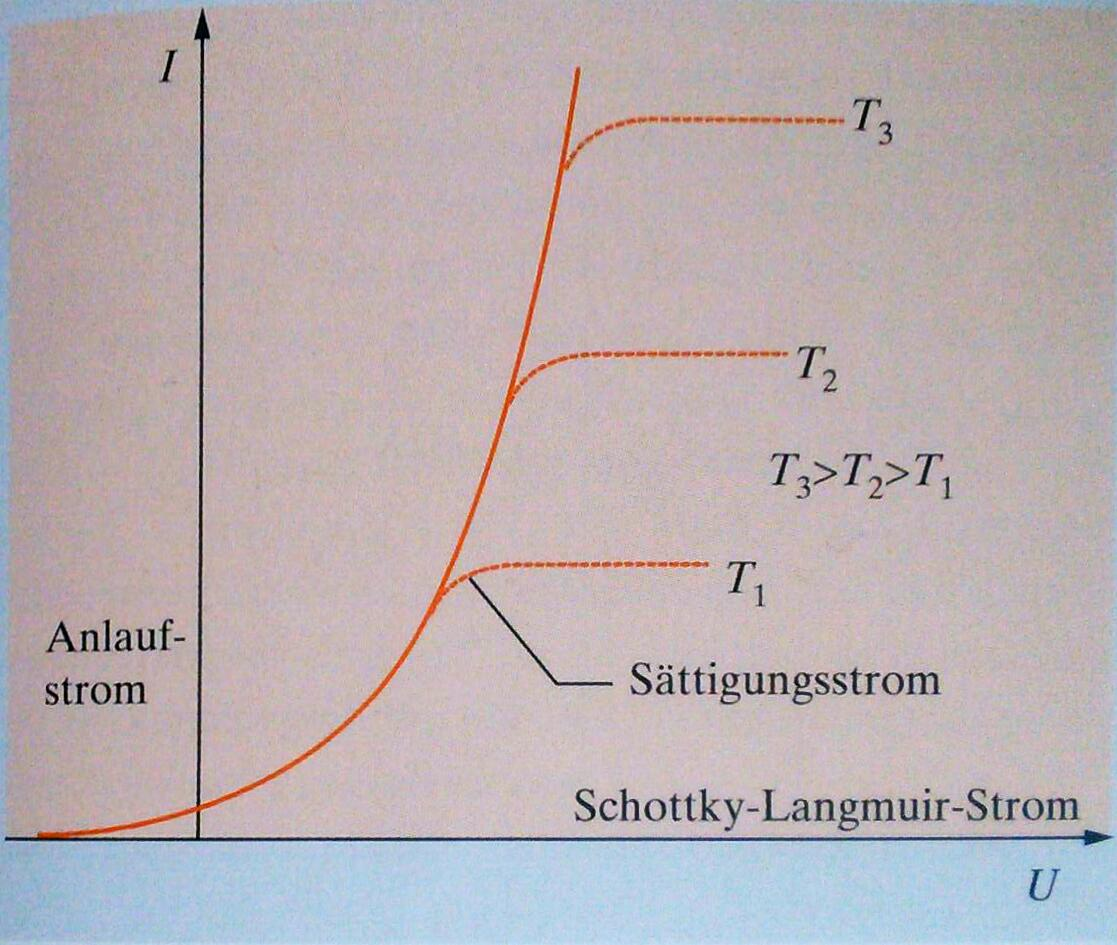
\includegraphics[width=0.4\textheight]{../figures/diode.jpg}
    \caption{Übergang des Anlaufstroms zur Raumladungsformel zum Sättigungsstrom. [Gerthsen]}
    \label{fig:diode}
  \end{figure}
